% Two-axes schematic of class-imbalance mitigation strategies (review comment C3).
% Each method is a MARKER placed at its exact rated level on both axes, 1:1 with the
% corrected C3 placement-evidence matrix (docs/C3_placement_matrix.md, Stage A sign-off):
%   x = pixel-level loss signal (algorithm-level); y = spatial-level exposure (data-level).
% Qualitative scale None=1, Low=3.5, Med=6, High=8.5; half-steps at 2.25 / 4.75 / 7.25.
% Shaded zones group the clusters; their edges sit at the midpoints between adjacent
% clusters' ratings: loss/both-axes split at y=Med(6.0) [KD Low-Med vs hard x minority
% Med-High]; exposure/both-axes split at x~6.7 [copy-paste Med vs hard x minority Med-High].
% Labels are offset for legibility and linked to their marker by a leader line, so marker
% position always equals the rated level. Encoding: marker fill = internal curation (teal)
% vs external supervision (orange); black ring = used in this study.
\documentclass[border=6pt]{standalone}
\usepackage[T1]{fontenc}
\usepackage{lmodern}
\usepackage{tikz}
\usetikzlibrary{positioning, arrows.meta, backgrounds}

\begin{document}

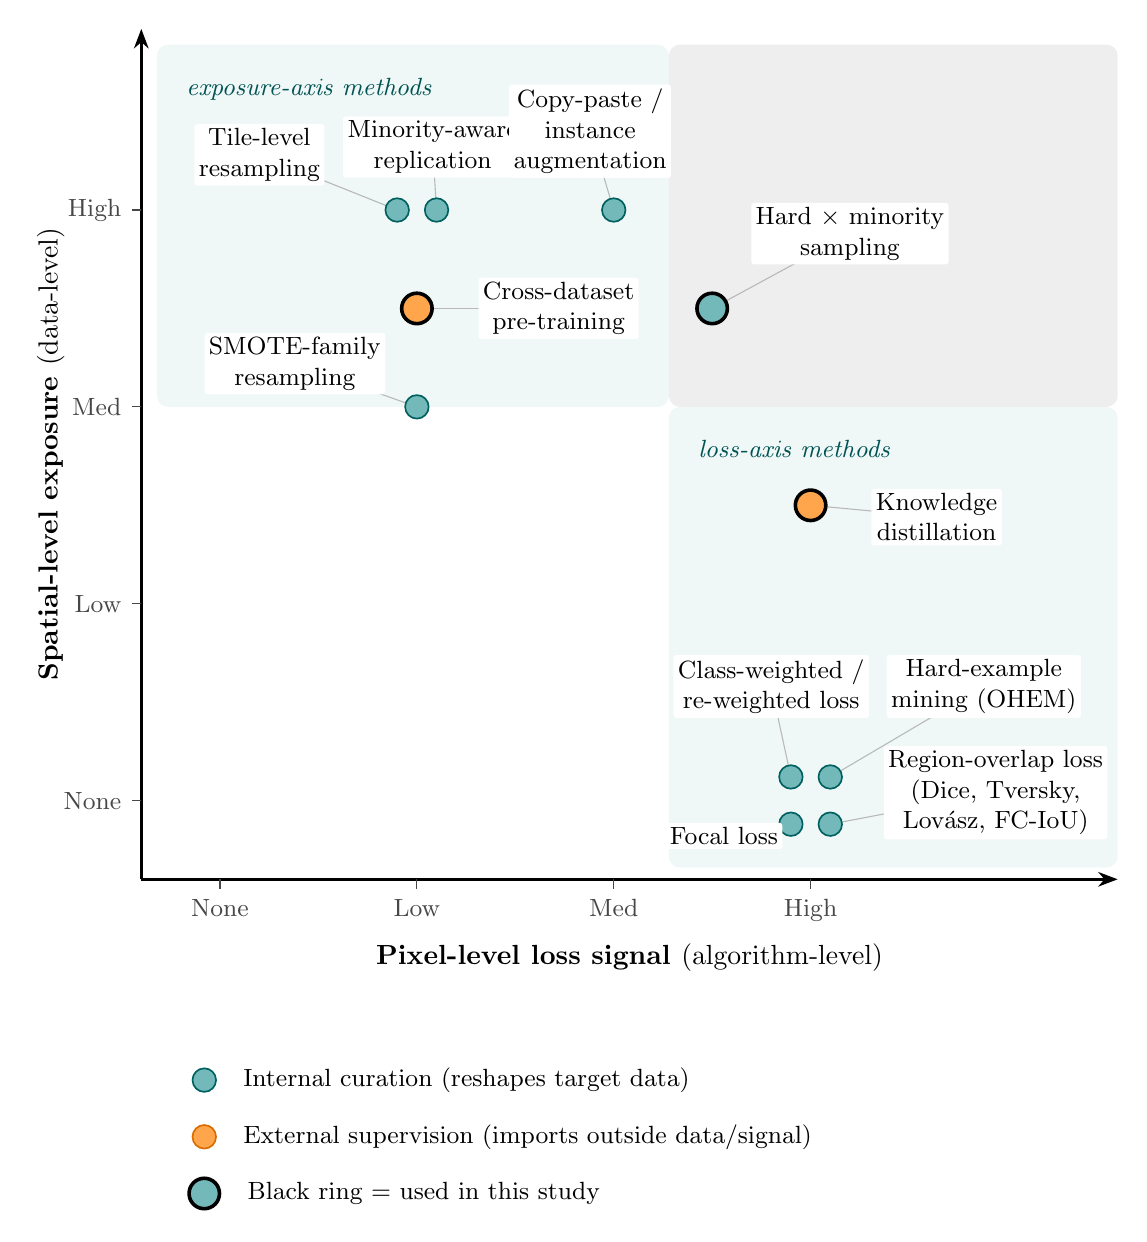
\begin{tikzpicture}[
  font=\normalsize,
  >=Stealth,
  mk/.style={circle, inner sep=0pt},
  mkint/.style={mk, minimum size=8.5pt, fill=teal!55, draw=teal!75!black, line width=0.6pt},
  mkext/.style={mk, minimum size=8.5pt, fill=orange!70, draw=orange!85!black, line width=0.6pt},
  mkintours/.style={mk, minimum size=11pt, fill=teal!55, draw=black, line width=1.3pt},
  mkextours/.style={mk, minimum size=11pt, fill=orange!70, draw=black, line width=1.3pt},
  lbl/.style={align=center, font=\small, fill=white, inner sep=1.6pt, rounded corners=1pt},
  lead/.style={gray!55, line width=0.4pt},
]

\def\xmax{12.4}
\def\ymax{10.8}

% ---- shaded zones (edges = midpoints between adjacent clusters' ratings) ----
\begin{scope}[on background layer]
  \fill[teal!6, rounded corners=4pt] (0.2,6.0) rectangle (6.7,10.6);    % exposure wall (top-left)
  \fill[teal!6, rounded corners=4pt] (6.7,0.15) rectangle (\xmax,6.0);  % loss wall (bottom-right)
  \fill[gray!13, rounded corners=4pt] (6.7,6.0) rectangle (\xmax,10.6); % sparse both-axes (top-right)
\end{scope}
\node[teal!65!black, anchor=north west, align=center, font=\small\itshape] at (0.45,10.3)
  {exposure-axis methods};
\node[teal!65!black, anchor=north west, align=center, font=\small\itshape] at (6.95,5.7)
  {loss-axis methods};

% ---- axes ----
\draw[->, line width=0.9pt] (0,0) -- (\xmax,0);
\draw[->, line width=0.9pt] (0,0) -- (0,\ymax);
\node[align=center, font=\bfseries] at (6.2,-1.0)
  {Pixel-level loss signal {\mdseries (algorithm-level)}};
\node[align=center, font=\bfseries, rotate=90] at (-1.15,5.4)
  {Spatial-level exposure {\mdseries (data-level)}};

% qualitative ticks
\foreach \x/\lab in {1/None, 3.5/Low, 6/Med, 8.5/High}{
  \draw[black!72] (\x,0) -- (\x,-0.12);
  \node[below, black!72, font=\small] at (\x,-0.13) {\lab};
}
\foreach \y/\lab in {1/None, 3.5/Low, 6/Med, 8.5/High}{
  \draw[black!72] (0,\y) -- (-0.12,\y);
  \node[left, black!72, font=\small] at (-0.13,\y) {\lab};
}

% ============================================================
% LEADER LINES (drawn first; opaque labels sit on top and hide the inner segment)
% ============================================================
\draw[lead] (7.4,0.55)  -- (8.25,0.7);   % focal
\draw[lead] (8.0,2.45)  -- (8.25,1.3);   % class-weighted
\draw[lead] (10.7,2.45) -- (8.75,1.3);   % ohem
\draw[lead] (10.85,1.1) -- (8.75,0.7);   % region-overlap
\draw[lead] (1.95,6.55) -- (3.5,6.0);    % smote
\draw[lead] (5.3,7.25)  -- (3.5,7.25);   % pre-training
\draw[lead] (1.5,9.2)   -- (3.25,8.5);   % tile-level
\draw[lead] (3.7,9.3)   -- (3.75,8.5);   % replication
\draw[lead] (5.7,9.5)   -- (6.0,8.5);    % copy-paste
\draw[lead] (9.0,8.2)   -- (7.25,7.25);  % hard x minority
\draw[lead] (10.1,4.6)  -- (8.5,4.75);   % kd

% ============================================================
% MARKERS at exact rated coordinates
% ============================================================
% pixel-loss family: 4 internal families all at High pixel / None spatial (tight rosette)
\node[mkint] at (8.25,0.7) {};   % focal
\node[mkint] at (8.75,0.7) {};   % region-overlap
\node[mkint] at (8.25,1.3) {};   % class-weighted
\node[mkint] at (8.75,1.3) {};   % ohem
% spatial wall (Low pixel column) + augmentation (Med pixel)
\node[mkint] at (3.5,6.0) {};    % smote      (Low / Med)
\node[mkint] at (3.25,8.5) {};   % tile-level (Low / High)
\node[mkint] at (6.0,8.5) {};    % copy-paste (Med / High)
% used in this study (black ring)
\node[mkextours] at (3.5,7.25) {};  % pre-training (Low / Med-High)
\node[mkint] at (3.75,8.5) {};  % replication  (Low / High) -- demoted: known internal-curation method, not used in this study
\node[mkintours] at (7.25,7.25) {}; % hard x minority (Med-High / Med-High)
\node[mkextours] at (8.5,4.75) {};  % kd (High / Low-Med)

% ============================================================
% LABELS (opaque, sitting on the tinted zones)
% ============================================================
\node[lbl] at (7.4,0.55)  {Focal loss};
\node[lbl] at (8.0,2.45)  {Class-weighted /\\re-weighted loss};
\node[lbl] at (10.7,2.45) {Hard-example\\mining (OHEM)};
\node[lbl] at (10.85,1.1) {Region-overlap loss\\(Dice, Tversky,\\Lov\'asz, FC-IoU)};
\node[lbl] at (1.95,6.55) {SMOTE-family\\resampling};
\node[lbl] at (5.3,7.25)  {Cross-dataset\\pre-training};
\node[lbl] at (1.5,9.2)   {Tile-level\\resampling};
\node[lbl] at (3.7,9.3)   {Minority-aware\\replication};
\node[lbl] at (5.7,9.5)   {Copy-paste /\\instance\\augmentation};
\node[lbl] at (9.0,8.2)   {Hard $\times$ minority\\sampling};
\node[lbl] at (10.1,4.6)  {Knowledge\\distillation};

% ============================================================
% LEGEND
% ============================================================
\begin{scope}[shift={(0.2,-2.55)}]
  \node[mkint] (lg1) at (0.6,0) {};
  \node[right=6pt of lg1, font=\small] {Internal curation (reshapes target data)};
  \node[mkext] (lg2) at (0.6,-0.72) {};
  \node[right=6pt of lg2, font=\small] {External supervision (imports outside data/signal)};
  \node[mkintours] (lg3) at (0.6,-1.44) {};
  \node[right=6pt of lg3, font=\small] {Black ring = used in this study};
\end{scope}

\end{tikzpicture}

\end{document}
